%
% Copyright 2018 Joel Feldman, Andrew Rechnitzer and Elyse Yeager.
% This work is licensed under a Creative Commons Attribution-NonCommercial-ShareAlike 4.0 International License.
% https://creativecommons.org/licenses/by-nc-sa/4.0/
%
\questionheader{ex:s1.10}

\noindent
Recall that we are using $\log x$ to denote the logarithm of $x$ with
base $e$. In other courses it is often denoted $\ln x$.


%%%%%%%%%%%%%%%%%%
\subsection*{\Conceptual}
%%%%%%%%%%%%%%%%%%
\begin{Mquestion}
Below are the graphs of four different quadratic functions. For each quadratic function, decide whether it is: (i) irreducible, (ii) the product of two distinct linear factors, or (iii) the product of a repeated linear factor (and possibly a constant).

\begin{tikzpicture}[scale=0.5]
\YEaxis{3}{3}
\draw[thick] plot[domain=-2.8:2.8](\x,{\x*\x/3});
\draw (-1.5,-3) node[below]{(a)};
\end{tikzpicture}\hfill
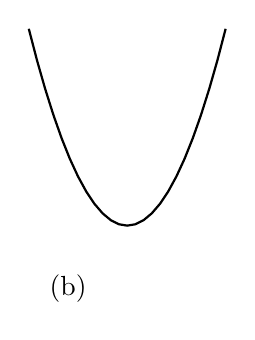
\begin{tikzpicture}[scale=0.5]
\YEaxis{3}{3}
\draw[thick] plot[domain=-5:5](\x/2,{\x*\x/5-2});
\draw (-1.5,-3) node[below]{(b)};
\end{tikzpicture}\hfill
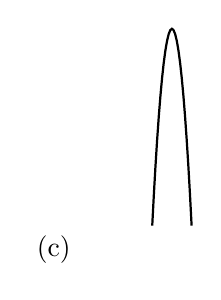
\begin{tikzpicture}[scale=0.5]
\YEaxis{3}{3}
\draw[thick] plot[domain=-5:5](\x/10+1.5,{2-\x*\x/5});
\draw (-1.5,-3) node[below]{(c)};
\end{tikzpicture}\hfill
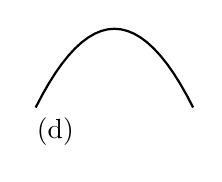
\begin{tikzpicture}[scale=0.5]
\YEaxis{3}{3}
\draw[thick] plot[domain=-2:2](\x,{-1-\x*\x/2});
\draw (-1.5,-3) node[below]{(d)};
\end{tikzpicture}


\end{Mquestion}
\begin{hint}
If a quadratic function can be factored as $(ax+b)(cx+d)$ for some constants $ a,b,c,d$, then it has roots $-\frac{b}{a}$ and $-\frac{d}{c}$.
\end{hint}
\begin{answer}
(a) (iii) \qquad (b) (ii) \qquad (c) (ii) \qquad (d) (i)
\end{answer}
\begin{solution}
If a quadratic function can be factored as $(ax+b)(cx+d)$ for some constants $ a,b,c,d$, then it has roots $-\frac{b}{a}$ and $-\frac{d}{c}$. So, if a quadratic function has no roots, it is irreducible: this is the case for the function in graph (d).

If a quadratic function has  two different roots, then $(ax+b) \neq \alpha(cx+d)$ for any constant $\alpha$. That is, the quadratic function is the product of distinct linear factors. This is the case for the functions graphed in (b) and (c), since these each have two distinct places where they cross the $x$-axis.

Finally, if a quadratic function has precisely one root, then $\frac{b}{a}=\frac{d}{c}$, so:
\begin{align*}
(ax+b)(cx+d)&=a(x+\tfrac{b}{a})(cx+d) = a(x+\tfrac{d}{c})(cx+d) = \tfrac{a}{c}(cx+d)(cx+d)
\end{align*}
That is, the quadratic function is the product of a repeated linear factor, and  a constant $\frac{a}{c}$ (which might simply be $\frac{a}{c}=1$).
\end{solution}
%%%%%%%%%%%%%%%%%%%


\begin{Mquestion}[2016Q4]
Write out the \textbf{general form} of the partial-fractions
decomposition of
$
\displaystyle\frac{x^3+3}{(x^2-1)^2(x^2+1)}
$.
You need not determine the values of any of the coefficients.
\end{Mquestion}

\begin{hint}
Review Equations~\eref{CLP101}{eq:PFdecompa} through \eref{CLP101}{eq:PFdecompd}
of the %\href{http://www.math.ubc.ca/%7Efeldman/m101/clp/clp_notes_101.pdf}{CLP-2 text}.
CLP-2 text.
Be careful to \emph{fully} factor the denominator.
\end{hint}

\begin{answer}
$\displaystyle\frac{A}{x-1}+\frac{B}{(x-1)^2}+\frac{C}{x+1}+\frac{D}{(x+1)^2}+\frac{Ex+F}{x^2+1} $
\end{answer}

\begin{solution}
Our first step is to fully factor the denominator:
\[(x^2-1)^2(x^2+1) = (x-1)^2(x+1)^2(x^2+1)\]
Once a term is linear, it can't be factored further; for quadratic terms, we should check that they are irreducible. Since $x^2+1$ has no real roots (we are familiar with its graph, which is entirely above the $x$-axis), it is irreducible, so now our denominator is fully factored.

\begin{align*}
\frac{x^3+3}{(x^2-1)^2(x^2+1)}
&=\frac{x^3+3}{(x-1)^2(x+1)^2(x^2+1)}\\
&=\frac{A}{x-1}+\frac{B}{(x-1)^2}+\frac{C}{x+1}+\frac{D}{(x+1)^2}+\frac{Ex+F}{x^2+1}
\end{align*}
Notice $(x-1)$ and $(x+1)$ are (repeated) linear factors, while $(x^2+1)$  is an irreducible quadratic factor. This accounts for the difference in the numerators of their corresponding terms.
\end{solution}

%%%%%%%%%%%%%%%%%%%


\begin{question}[2016Q4]\label{prob_s1.10:sneaky}
Find the coefficient of $\displaystyle \frac{1}{x-1}$ in the partial
fraction decomposition of $\displaystyle\frac{3x^3-2x^2+11}{x^2(x-1)(x^2+3)}$.
\end{question}

\begin{hint}
Review   Example \eref{CLP101}{eg:PFa}
in the %\href{http://www.math.ubc.ca/%7Efeldman/m101/clp/clp_notes_101.pdf}{CLP-2 text}.
CLP-2 text. Is the ``Algebraic Method'' or the ``Sneaky Method'' going to be easier?
\end{hint}

\begin{answer}
$3$
\end{answer}

\begin{solution}
The partial fraction decomposition has the form
\begin{align*}
  \frac{3x^3-2x^2+11}{x^2(x-1)(x^2+3)} = \frac A{x-1} + \text{various terms}
\end{align*}
When we multiply through by the original denominator, this becomes
\begin{align*}
{3x^3-2x^2+11} = {x^2(x^2+3)}A + (x-1)(\text{other terms}).
\end{align*}
Evaluating both sides at $x=1$ yields $3\cdot1^3-2\cdot1^2+11=1^2(1^2+3)A+0$, or $A=3$.
\end{solution}

%%%%%%%%%%%%%%%%%%

\begin{comment}
\begin{question}
Find the numerator of $\displaystyle \frac{P(x)}{ 2x^2+1}$ in the partial
fraction decomposition of $\displaystyle\frac{10x^3-46x^2+17x-40}{(x-3)^2(2x^2+1) }$.
\end{question}
\begin{hint}
Review   Example \eref{CLP101}{eg:PFa}
in the %\href{http://www.math.ubc.ca/%7Efeldman/m101/clp/clp_notes_101.pdf}{CLP-2 text}.
CLP-2 text. The  ``Algebraic Method'' and the ``Sneaky Method'' are about the same length in this problem--it's good to practice both.
\end{hint}
\begin{answer}
$-2$
\end{answer}
\begin{solution}
We notice the denominator is already factored into linear and irreducible quadratic factors. (We can check that $2x^2+1$ is irreducible by noticing that the graph never crosses the $x$-axis, or by checking that the quadratic equation gives no real roots.) So, the partial fraction decomposition has the form
\begin{align*}
\frac{10x^3-46x^2+17x-40}{(x-3)^2(2x^2+1) }&=\frac{A}{x-3}+\frac{B}{(x-3)^2}
+\frac{Cx+D}{2x^2+1}
\intertext{ We multiply through by the original denominator.}
10x^3-46x^2+17x-40&=
A(x-3)(2x^2+1)+B(2x^2+1)+(Cx+D)(x-3)^2
\end{align*}

\begin{description}
\item[Solution 1:]
Let's try the ``Sneaky Method" that worked so well in Question~\ref{prob_s1.10:sneaky}. Setting $x=3$ makes every term except the one with $B$ disappear--but we're looking for $C$ and $D$. The ``Sneaky Method" doesn't solve everything right away, but it gives us  $B$.
\begin{align*}
10(27)-46(9)+17(3)-40&=B(2(9)+1)\\
B&=-7
\intertext{This allows us to simplify our expression somewhat.}
10x^3-32x^2+17x-33&=
A(x-3)(2x^2+1)+(Cx+D)(x-3)^2\\
&=(x-3)\big(A(2x^2+1)+(Cx+D)(x-3)\big)
\intertext{Since $x-3$ is a factor of the right-hand side of the equation, it must also be  a factor on the left. Long division shows us how to to cancel it out.}
\intertext{\centering\polylongdiv{10x^3-32x^2+17x-33}{x-3}}
(x-3)(10x^2-2x+11)
&=(x-3)\big(A(2x^2+1)+(Cx+D)(x-3)\big)\\
10x^2-2x+11&=A(2x^2+1)+(Cx+D)(x-3)
\intertext{Plugging in $x=3$, we see}
10(9)-2(3)+11&=A(2(9)+1)\\
A&=5
\intertext{Again, this allows us to simplify our equation.}
10x^2-2x+11&=5(2x^2+1)+(Cx+D)(x-3)\\
-2x+6&=(Cx+D)(x-3)\\
-2(x-3)&=(Cx+D)(x-3)\\
-2&=Cx+D\\
C&=0,\quad D=-2
\end{align*}
So, the term we're looking for is $\dfrac{-2}{2x^2+1}$.
\item[Solution 2:] Let's go through the algebra method. This requires rearranging the right-hand side of our equation.
\begin{align*}10x^3-&46x^2+17x-40=
A(x-3)(2x^2+1)+B(2x^2+1)+(Cx+D)(x-3)^2
\\&=A(2x^3-6x^2+x-3)+B(2x^2+1)+C(x^3-6x^2+9x)+D(x^2-6x+9)\\
&=x^3(2A+C)+x^2(-6A+2B-6C+D)+x(A+9C-6D)+(-3A+B+9D)
\end{align*}
By matching the  coefficients of corresponding powers of $x$, we make a system of four equations.
\begin{align*}
(1)\quad 10&=2A+C & (2)\quad -46&=-6A+2B-6C+D\\
(3)\quad 17&=A+9C-6D & (4)\quad -40&=-3A+B+9D
\end{align*}

\begin{itemize}
\item Equation 1 gives us $C$ in terms of $A$: $C = 10-2A$
\item Substituting this into the remaining equations eliminates $C$ from them:
\begin{alignat*}{3}
(2)&&-46&=-6A+2B-6(10-2A)+D\\
&\Rightarrow& 14&=6A+2B+D\\
(3)&&\quad 17&=A+9(10-2A)-6D\\
&\Rightarrow& -73&=-17A-6D\\
(4)&&-40&=-3A+B+9D
\end{alignat*}
\item Now, Equation (2) gives us $D$ in terms of $A$ and $B$: $D=14-6A-2B$.
\item Substituting this into the remaining equations eliminates $D$.
\begin{alignat*}{3}
(3)&&\quad  -73&=-17A-6(14-6A-2B)\\
&\Rightarrow& 11&=19A+12B\\
(4)&&-40&=-3A+B+9(14-6A-2B)\\
&\Rightarrow& -166&=-57A-17B
\end{alignat*}
\item Equation (3) gives us $B$ in terms of $A$: $B = \frac{11}{12} - \frac{19}{12}A$.
\item Substituting this into Equation (4) gives us $A$:
\begin{alignat*}{3}
(4)&&-166&=-57A-17\left( \frac{11}{12} - \frac{19}{12}A\right)\\
&\Rightarrow& A&=5
\end{alignat*}
\item Since $B= \frac{11}{12} - \frac{19}{12}A$, $B=-7$.
\item Since $D = 14-6A-2B$, $D=-2$.
\item Since $C=10-2A$, $C=0$.
\end{itemize}
So, the term we're looking for is
\[\frac{Cx+D}{2x^2+1} = \frac{-2}{2x^2+1}\]decomposition
\end{description}
Remark: for more complicated partial fraction decompositions (like this one), once you're comfortable with both methods, you'll be able to blend them. For example, in Solution 1, it was very easy to find $B=-7$, but then there was long division, which is time-consuming. We could have switched over to the algebra method here, but kept the result $B=-7$ to simplify our equation.
\end{solution}
\end{comment}

%%%%%%%%%%%%%%%%%%%

\begin{Mquestion}
Re-write the following rational functions as the sum of a polynomial and a rational function whose numerator has a strictly smaller degree than its denominator. (Remember our method of partial fraction decomposition of a rational function only works when the degree of the numerator is strictly smaller than the degree of the denominator.)
\begin{enumerate}[(a)]
\item $\dfrac{x^3+2x+2}{x^2+1}$
\item $\dfrac{15x^4+6x^3+34x^2+4x+20}{5x^2+2x+8}$
\item $\dfrac{2x^5+9x^3+12x^2+10x+30}{2x^2+5}$
\end{enumerate}

\end{Mquestion}
\begin{hint}
For each part,  use long division as in Example~\eref{CLP101}{eg:PFdd} of the CLP-2 text.
\end{hint}
\begin{answer}
(a) $\displaystyle\frac{x^3+2x+2}{x^2+1} = x+\frac{x+2}{x^2+1}$\\[10pt]
(b) $\displaystyle\dfrac{15x^4+6x^3+34x^2+4x+20}{5x^2+2x+8} = 3x^2+2+\frac{4}{5x^2+2x+8}$\\[10pt]
(c) $\displaystyle\dfrac{2x^5+9x^3+12x^2+10x+30}{2x^2+5}=x^3+2x+6$
\end{answer}
\begin{solution}
\begin{enumerate}[(a)]
\item We start by dividing. The leading term of the numerator is $x$ times the leading term of the denominator. The remainder is $x+2$.
\begin{center}\polylongdiv{x^3+2x+2}{x^2+1}
\end{center}
That is, $x^3+2x+2 = x(x^2+1)+(x+2)$. So,
 \[\frac{x^3+2x+2}{x^2+1} = x+\frac{x+2}{x^2+1}\]

\item We start by dividing. The leading term of the numerator is $3x^2$ times the leading term of the denominator.
\begin{center}\polylongdiv[stage=4]{15x^4+6x^3+34x^2+4x+20}{5x^2+2x+8}
\end{center}
Then $5x^2$ goes into $10x^2$ twice, so
\begin{center}\polylongdiv[stage=7]{15x^4+6x^3+34x^2+4x+20}{5x^2+2x+8}
\end{center}
Our remainder is 4. That is,

\[\dfrac{15x^4+6x^3+34x^2+4x+20}{5x^2+2x+8} = 3x^2+2+\frac{4}{5x^2+2x+8}.\]

\item
We start by dividing. The leading term of the numerator is $x^3$ times the leading term of the denominator.

\begin{center}\polylongdiv[stage=4]{2x^5+9x^3+12x^2+10x+30}{2x^2+5}
\end{center}

Then $2x^2(2x)$ gives us $4x^3$.
\begin{center}\polylongdiv[stage=7]{2x^5+9x^3+12x^2+10x+30}{2x^2+5}
\end{center}

Finally, $2x^2$ goes into $12x^2$ six times.
\begin{center}\polylongdiv[]{2x^5+9x^3+12x^2+10x+30}{2x^2+5}
\end{center}

Since there is no remainder,
\[\dfrac{2x^5+9x^3+12x^2+10x+30}{2x^2+5}=x^3+2x+6\]

Remark: if we wanted to be pedantic about the question statement, we could write our final answer as $x^3+2x+6+\frac{0}{x}$, so that we are indeed adding a polynomial to a rational function whose numerator has degree strictly smaller than its denominator.
\end{enumerate}

\end{solution}
%%%%%%%%%%%%%%%%%%%



\begin{question} Factor the following polynomials into linear and irreducible factors.
\begin{enumerate}[(a)]
\item $5x^3-3x^2-10x+6$
\item $x^4-3x^2-5$
\item $x^4-4x^3-10x^2-11x-6$
\item $2x^4+12x^3-x^2-52x+15$
\end{enumerate}
\end{question}
\begin{hint}
(a) Look for a pattern you can exploit to factor out a linear term.\\
(b) If you set $y=x^2$, this is quadratic. Remember $(x^2-a)= (x+\sqrt{a})(x-\sqrt{a})$ as long as $a$ is positive.\\
(c),(d) Look for integer roots, then use long division.
\end{hint}
\begin{answer}
(a) $5x^3-3x^2-10x+6=(x+\sqrt{2})(x-\sqrt{2})(5x-3)$\\[10pt]
(b)  $x^4-3x^2-5=\displaystyle\left(x+\sqrt{\frac{3+\sqrt{29}}{2}}\right)\left(x-\sqrt{\frac{3+\sqrt{29}}{2}}\right)\left(x^2+\frac{\sqrt{29}-3}{2}\right)$\\[10pt]
(c) $x^4-4x^3-10x^2-11x-6 = (x+1)(x-6)(x^2+x+1)$\\
(d) $2x^4+12x^3-x^2-52x+15= (x+3)(x+5)\left(x-(2+\sqrt2)\right)\left(x-(2-\sqrt2)\right)$
\end{answer}
\begin{solution}
\begin{enumerate}[(a)]
\item The polynomial $5x^3-3x^2-10x+6$ has a repeated pattern: the ratio of the first two coefficients is the same as the ratio of the last two coefficients. We can use this to factor.
\begin{align*}
5x^3-3x^2-10x+6&=x^2(5x-3)-2(5x-3) = (x^2-2)(5x-3)\\
&=(x+\sqrt{2})(x-\sqrt{2})(5x-3)
\end{align*}


\item The polynomial $x^4-3x^2-5$ has only even powers of $x$, so we can (temporarily) replace them with $x^2=y$ to turn our quartic polynomial into a quadratic.
\begin{align*}
x^4-3x^2-5&=y^2-3y-5
\intertext{There's no obvious factoring here, but we can find its roots, if any, using the quadratic equation.}
y&=\frac{3\pm\sqrt{3^2-4(1)(-5)}}{2}\\
&=\frac{3\pm\sqrt{29}}{2}\\
\mbox{So,}\qquad y^2-3y-5&=\left(y-\frac{3+\sqrt{29}}{2}\right)\left(y-\frac{3-\sqrt{29}}{2}\right)\\
\mbox{Therefore,}\qquad x^4-3x^2-5&=\left(x^2-\frac{3+\sqrt{29}}{2}\right)\left(x^2-\frac{3-\sqrt{29}}{2}\right)
\intertext{We'd like to use the difference of two squares to factor these quadratic expressions. For this to work, the constants must be positive (so their square roots are real). Since $\sqrt{29}>3$, only the first quadratic is factorable. The other is irreducible--it's always positive, so it had no roots.}
 x^4-3x^2-5&=\left(x+\sqrt{\frac{3+\sqrt{29}}{2}}\right)\left(x-\sqrt{\frac{3+\sqrt{29}}{2}}\right)\left(x^2+\frac{\sqrt{29}-3}{2}\right)
\end{align*}



\item Without seeing any obvious patterns, we start hunting for roots. Since we have all integer coefficients, if there are any integer roots, they will divide our constant term, $-6$. So, our candidates for roots are $\pm1,\,\pm2,\,\pm3,$ and $\pm6$. To save time, we don't need to know exactly the value of our polynomial at these points: only whether or not it is 0. Write $f(x) = x^4  - 4x^3 - 10x^2 - 11x - 6$.
\begin{align*}
\color{red}f(-1)&\color{red}=0&
f(-2)&\neq 0&
f(-3)&\neq 0&
f(-6)&\neq 0\\
f(1)&\neq 0&
f(2)&\neq 0&
f(3)&\neq 0&
\color{red}f(6)&\color{red}= 0
\end{align*}
Since $x=-1$ and $x=6$ are roots of our polynomial, it has factors $(x+1)$ and $(x-6)$. Note $(x+1)(x-6) = x^2-5x-6$. We use long division to figure out what else is lurking in our polynomial.
\begin{center}
 \polylongdiv{x^4-4x^3-10x^2-11x-6}{x^2-5x-6}\end{center}

 So, $x^4-4x^3-10x^2-11x-6 = (x+1)(x-6)(x^2+x+1)$.

 We should check whether $x^2+x+1$ is reducible or not. If we try to find its roots with the quadratic equation, we get $\dfrac{-1\pm\sqrt{-3}}{2}$, which are not real numbers. So, we're at the end of our factoring.

 \item Without seeing any obvious patterns, we start hunting for roots. Since we have all integer coefficients, if there are any integer roots, they will divide our constant term, $-15$. So, our candidates for roots are $\pm1,\,\pm3,\,\pm5,$ and $\pm15$.
Write $f(x) = 2x^4  + 12x^3 - x^2 - 52x + 15$.
\begin{align*}
f(-1)&\neq 0&
\color{red}f(-3)&\color{red}=0&
\color{red}f(-5)&\color{red}= 0&
f(-5)&\neq 0\\
f(1)&\neq 0&
f(3)&\neq 0&
f(5)&\neq 0&
f(15)&\neq 0&
\end{align*}
Since $x=-3$ and $x=-5$ are roots of our polynomial, it has factors $(x+3)$ and $(x+5)$. Note $(x+3)(x+5) = x^2+8x+15$. We use long division to move forward.

\begin{center}
 \polylongdiv{2x^4+12x^3-x^2-52x+15}{x^2+8x+15}\end{center}

 So, $2x^4+12x^3-x^2-52x+15= (x+3)(x+5)(2x^2-4x+1)$.

 We should check whether $2x^2-4x+1$ is reducible or not. There's not an obvious way to factor it, but we can  use the quadratic equation. This gives us roots
 $\dfrac{4\pm\sqrt{16-8}}{2}=2\pm\sqrt2$. So, we have two more linear factors.

Specifically:  $2x^4+12x^3-x^2-52x+15= (x+3)(x+5)\left(x-(2+\sqrt2)\right)\left(x-(2-\sqrt2)\right)$.

\end{enumerate}

\end{solution}
%%%%%%%%%%%%%%%%%%%


\begin{question}
Here is a fact:
\begin{quote}
 \color{blue}
Suppose we have a rational function with a repeated linear factor $(ax+b)^n$ in the denominator, and the degree of the numerator is strictly less than the degree of the denominator. In the partial fraction decomposition, we can replace the terms
\begin{equation}\frac{A_1}{ax+b} + \frac{A_2}{(ax+b)^2}+\frac{A_3}{(ax+b)^3}+\cdots+
\frac{A_n}{(ax+b)^n}\tag{1}\end{equation}
with the single term
\begin{equation}\frac{B_1+B_2x+B_3x^2+\cdots + B_{n}x^{n-1}}{(ax+b)^n}\tag{2}\end{equation}
and still be guaranteed to find a solution.\color{black}\end{quote}

Why do we use the sum in (1), rather than the single term in (2), in partial fraction decomposition?
\end{question}
\begin{hint}
Why do we do partial fraction decomposition at all?
\end{hint}
\begin{answer}
The goal of partial fraction decomposition is to write our integrand in a form that is easy to integrate. The antiderivative of (1) can be easily determined with the substitution $u=(ax+b)$. It's less clear how to find the antiderivative of (2).
\end{answer}
\begin{solution}
The goal of partial fraction decomposition is to write our integrand in a form that is easy to integrate. The antiderivative of (1) can be easily determined with the substitution $u=(ax+b)$. It's less clear how to find the antiderivative of (2).
\end{solution}
%%%%%%%%%%%%%%%%%%%




%%%%%%%%%%%%%%%%%%
\subsection*{\Procedural}
%%%%%%%%%%%%%%%%%%

\begin{question}[2013A]\label{prob_s1.10:x+x^2}
Evaluate $\displaystyle\int_1^2 \frac{\dee{x}}{x+x^2}$.
\end{question}

\begin{hint}
What is the title of this section?
\end{hint}

\begin{answer}
$\displaystyle\log\frac{4}{3}$
\end{answer}

\begin{solution}
The integrand is a rational function, so it's a candidate for partial fraction. We quickly rule out any obvious substitution or integration by parts, so we go ahead with the decomposition.


We start by expressing the integrand,
i.e. the fraction $\frac{1}{x+x^2}=\frac{1}{x(1+x)}$, as a linear
combination of the simpler fractions  $\frac{1}{x}$ and $\frac{1}{x+1}$
(which we already know how to integrate). We will have
\begin{align*}
\frac{1}{x+x^2}=\frac{1}{x(1+x)} = \frac{a}{x} + \frac{b}{x+1}
=\frac{a(x+1) +bx}{x(1+x)}
\end{align*}
The fraction on the left hand side is the same as the fraction
on the right hand side if and only if the numerator on the left
hand side, which is $1 = 0x + 1$, is equal to the numerator on the
right hand side, which is $a(x+1)+bx = (a+b)x +a$. This in turn
is the case if and only of $a=1$ (i.e. the constant terms are
the same in the two numerators) and $a+b=0$ (i.e. the coefficients
of $x$ are the same in the two numerators). So $a=1$ and $b=-1$.
Now we can easily evaluate the integral
\begin{align*}
\int_1^2 \frac{\dee{x}}{x+x^2}
&=\int_1^2 \frac{\dee{x}}{x(x+1)}
=\int_1^2 \Big(\frac{1}{x}-\frac{1}{x+1}\Big)\,\dee{x}
=\Big[\log x-\log(x+1)\Big]_1^2\\
&=\log 2-\log\frac{3}{2}
=\log\frac{4}{3}
\end{align*}
\end{solution}

\begin{question}[2015A]
Calculate $\displaystyle \int \frac{1}{x^4+x^2}\,\dee{x}$.
\end{question}

\begin{hint}
You can save yourself some work in developing your partial fraction decomposition
by renaming $x^2$ to $y$ and comparing the result with Question~\ref{prob_s1.10:x+x^2}.
\end{hint}

\begin{answer}
$-\dfrac{1}{x}-\arctan x+C$
\end{answer}

\begin{solution}
We'll first do a partial fraction decomposition. The sneaky
way is to temporarily rename $x^2$ to $y$. Then $x^4+x^2=y^2+y$
and
\begin{equation*}
\frac{1}{x^4+x^2} = \frac{1}{y(y+1)}
  =\frac{1}{y}-\frac{1}{y+1}
\end{equation*}
  as we found in Question~\ref{prob_s1.10:x+x^2}.
Now we restore $y$ to $x^2$.
\begin{align*}
\int \frac1{x^4+x^2}\,\dee{x}
=\int \Big(\frac{1}{x^2}-\frac{1}{x^2+1}\Big)\,\dee{x}
=-\frac{1}{x}-\arctan x+C
\end{align*}

\end{solution}
%%%%%%%%%%%%%%%%%%%

\begin{Mquestion}[2016A]
Calculate $\displaystyle \int \frac{12x+4}{(x-3)(x^2+1)}\,dx$.
\end{Mquestion}

\begin{hint}
Review Steps 3 (particularly the ``Sneaky Method'') and 4 of
Example \eref{CLP101}{eg:PFc} in the CLP-2 text.
\end{hint}

\begin{answer}
$4 \log |x-3| - 2 \log (x^2 + 1) + C$
\end{answer}

\begin{solution}
The integrand is of the form $N(x)/D(x)$ with $D(x)$ already factored
and $N(x)$ of lower degree. We immediately look for a partial fraction decomposition:
\begin{equation*}
\frac{12x+4}{(x-3)(x^2+1)} = \frac{A}{x-3} + \frac{Bx+C}{x^2+1}.
\end{equation*}
Multiplying through by the denominator yields
\begin{align}
12x+4 &= A(x^2+1) + (Bx+C)(x-3)
\tag{$*$}
\end{align}
Setting $x=3$ we find:
\begin{align*}
   36 +4 = A(9 + 1) + 0 \implies 40 =10A  \implies \color{red}A = 4
\end{align*}
Substituting $A=4$ in $(*)$ gives
\begin{align*}
12x+4 = 4(x^2+1) + (Bx+C)(x-3)
  &\implies   -4x^2+12 x =(x-3)(Bx + C) \\
  &\implies   (-4x)(x-3)=(Bx + C)(x-3) \\
  & \implies  \color{red}B=-4,~C=0
\end{align*}
So we have found that $A=4$, $B=-4$, and $C=0$. Therefore
\begin{align*}
  \int \frac{12x+4}{(x-3)(x^2+1)} \,dx &= \int \bigg( \frac{4}{x-3} - \frac{4x}{x^2+1} \bigg) \,dx \\
   &=  4 \log |x-3| - 2 \log (x^2 + 1) + C
\end{align*}
The second integral was found just by guessing an antiderivative.
Alternatively, one could use the substitution $u=x^2+1$, $\dee{u}=2x\,\dee{x}$.
\end{solution}
%%%%%%%%%%%%%%%%%%%


\begin{question}[2016Q4]
Evaluate the following indefinite integral using partial fraction:
\begin{align*}
F(x) = \int \frac{3x^2 -4}{(x-2)(x^2+4)}\,\dee{x} .
\end{align*}
\end{question}

\begin{hint}
Review Steps 3 (particularly the ``Sneaky Method'') and 4 of
Example \eref{CLP101}{eg:PFc}
in the %\href{http://www.math.ubc.ca/%7Efeldman/m101/clp/clp_notes_101.pdf}{CLP-2 text}.
CLP-2 text. Remember $\diff{}{x}\{\arctan x\} = \frac{1}{1+x^2}$.
\end{hint}

\begin{answer}
$ F(x) = \log |x-2| + \log |x^2+4| + 2\arctan (x/2) + D$
\end{answer}

\begin{solution}
The integrand is of the form $N(x)/D(x)$ with $D(x)$ already factored
and $N(x)$ of lower degree. With no obvious substitution available, we look for a partial fraction decomposition.
\begin{align*}
\frac{3x^2 -4}{(x-2)(x^2+4)} = \frac{A}{x-2} + \frac{Bx + C}{x^2+4}
\end{align*}
Multiplying through by the denominator gives
\begin{align}
3x^2 -4 = A(x^2+4) + (Bx + C)(x-2)
\tag{$*$}
\end{align}
Setting $x=2$ we find:
\begin{align*}
   12 -4 = A(4 + 4) + 0 \implies 8 =8A  \implies \color{red}A = 1
\end{align*}
Substituting $A=1$ in $(*)$ gives
\begin{align*}
 3x^2 -4  = (x^2+4) + (x-2)(Bx + C)
  &\implies   2x^2-8 =(x-2)(Bx + C) \\
  &\implies   (x-2)(2x+4)=(x-2)(Bx + C) \\
  & \implies \color{red} B=2,~C=4
\end{align*}
Thus, we have:
\begin{align*}
 \frac{3x^2 -4}{(x-2)(x^2+4)} = \frac{1}{x-2} + \frac{2x + 4}{x^2+4} = \frac{1}{x-2} + \frac{2x }{x^2+4} + \frac{4}{x^2+4 }
\end{align*}
The first two of these are directly integrable:
\begin{align*}
  F(x) = \log |x-2| + \log |x^2+4| + \int \frac{4}{x^2+4}\,\dee{x}
\end{align*}
(The second integral was found just by guessing an antiderivative.
Alternatively, one could use the substitution $u=x^2+4$, $\dee{u}=2x\,\dee{x}$.)
For the final integral, we substitute: $x = 2y$,
$\dee{x} = 2\dee{y}$, and see that:
\begin{align*}
  \int \frac{4}{x^2+4}\,\dee{x}  = 2 \int \frac{1}{y^2 + 1}\,dy = 2 \arctan y + D = 2\arctan (x/2) + D
\end{align*}
for any constant $D$. All together we have:
\begin{align*}
   F(x) = \log |x-2| + \log |x^2+4| + 2\arctan (x/2) + D
\end{align*}
\end{solution}
%%%%%%%%%%%%%%%%%%%%%%%%%%%%%%%%%%%%%%

\begin{question}[M105 2014A]
Evaluate $\displaystyle\int \frac{x-13}{x^2-x-6}\dee{x}$.
\end{question}

\begin{hint}
Fill in the blank: the integrand is a $\underbar{\ \ \ \ \ \ \ \ }$ function.
\end{hint}

\begin{answer}
$-2\log|x-3|+3\log|x+2|+C$
\end{answer}

\begin{solution}
This integrand is a rational function, with no obvious substitution. This sure looks like a partial fraction problem. Let's go through our protocol.
\begin{itemize}
\item
The degree of the numerator $x-13$ is one, which is strictly smaller
than the dergee of the denominator $x^2-x-6$, which is two. So we don't need long division to pull out a polynomial.

\item
Next we factor the denominator.
\begin{align*}
x^2-x-6 = (x-3)(x+2)
\end{align*}

\item
Next we find the partial fraction decomposition of the integrand. It is
of the form
\begin{align*}
\frac{x-13}{(x-3)(x+2)}
=\frac{A}{x-3} + \frac{B}{x+2}
\end{align*}
To find $A$ and $B$, using the sneaky method, we cross multiply by the
denominator.
\begin{align*}
x-13 = A(x+2) + B(x-3)
\end{align*}
Now we can find $A$ by evaluating at $x=3$
\begin{align*}
3-13 = A(3+2) + B(3-3)
\implies \color{red}A=-2
\end{align*}
and find $B$ by evaluating at $x=-2$.
\begin{align*}
-2-13 = A(-2+2) + B(-2-3)
\implies \color{red}B=3
\end{align*}
(Hmmm. $A$ and $B$ are nice round numbers. Sure looks like a rigged exam or
homework question.) Our partial fraction decomposition is
\begin{align*}
\frac{x-13}{(x-3)(x+2)}
=\frac{-2}{x-3} + \frac{3}{x+2}
\end{align*}
As a check, we recombine the right hand side and make sure that
it matches the left hand side.
\begin{align*}
\frac{-2}{x-3} + \frac{3}{x+2}
=\frac{-2(x+2)+3(x-3)}{(x-3)(x+2)}
=\frac{x-13}{(x-3)(x+2)}
\end{align*}

\item
Finally, we evaluate the integral.
\begin{align*}
\int \frac{x-13}{x^2-x-6}\dee{x}
=\int\bigg(\frac{-2}{x-3} + \frac{3}{x+2}\bigg)\dee{x}
=-2\log|x-3|+3\log|x+2|+C
\end{align*}

\end{itemize}


\end{solution}
%%%%%%%%%%%%%%%%%%%

\begin{question}[2014D]
Evaluate $\displaystyle\int \frac{5x+1}{x^2+5x+6}\dee{x}$.
\end{question}

\begin{hint}
The integrand is yet another $\underbar{\ \ \ \ \ \ \ \ }$ function.
\end{hint}

\begin{answer}
$ -9\log|x+2|+14\log|x+3| +C$
\end{answer}

\begin{solution}
Again, this sure looks like a partial fraction problem. So let's go
through our protocol.
\begin{itemize}
\item
The degree of the numerator $5x+1$ is one, which is strictly smaller
than the dergee of the denominator $x^2+5x+6$, which is two. So we do not
long divide to pull out a polynomial.

\item
Next we factor the denominator.
\begin{align*}
x^2+5x+6 = (x+2)(x+3)
\end{align*}

\item
Next we find the partial fraction decomposition of the integrand. It is
of the form
\begin{align*}
\frac{5x+1}{(x+2)(x+3)}
=\frac{A}{x+2} + \frac{B}{x+3}
\end{align*}
To find $A$ and $B$, using the sneaky method, we cross multiply by the
denominator.
\begin{align*}
5x+1= A(x+3) + B(x+2)
\end{align*}
Now we can find $A$ by evaluating at $x=-2$
\begin{align*}
-10+1 = A(-2+3) + B(-2+2)
\implies\color{red} A=-9
\end{align*}
and find $B$ by evaluating at $x=-3$.
\begin{align*}
-15+1 = A(-3+3) + B(-3+2)
\implies\color{red} B=14
\end{align*}
So our partial fraction decomposition is
\begin{align*}
\frac{5x+1}{(x+2)(x+3)}
=\frac{-9}{x+2} + \frac{14}{x+3}
\end{align*}
As a check, we recombine the right hand side and make sure that
it matches the left hand side
\begin{align*}
\frac{-9}{x+2} + \frac{14}{x+3}
=\frac{-9(x+3)+14(x+2)}{(x+2)(x+3)}
=\frac{5x+1}{(x+2)(x+3)}
\end{align*}

\item
Finally, we evaluate the integral
\begin{align*}
\int \frac{5x+1}{x^2+5x+6}\dee{x}
=\int\bigg(\frac{-9}{x+2} + \frac{14}{x+3}\bigg)\dee{x}
=-9\log|x+2|+14\log|x+3|+C
\end{align*}

\end{itemize}


\end{solution}


%%%%%%%%%%%%%%%%%%%



\begin{Mquestion}
Evaluate $\displaystyle\int \frac{5x^2-3x-1}{x^2-1}~\dee{x}$.
\end{Mquestion}
\begin{hint}
Since the degree of the numerator is the same as the degree of the denominator, we can't do our partial fraction decomposition before we simplify the integrand.
\end{hint}
\begin{answer}
$\displaystyle5x+\frac{1}{2}\log|x-1| - \frac{7}{2}\log|x+1|+C$
\end{answer}
\begin{solution}
We have a rational function with no obvious substitution, so let's use partial fraction decomposition.
\begin{itemize}
\item Since the degree of the numerator is the same as the degree of the denominator, we need to pull out a polynomial.

\begin{center}
\polylongdiv{3x^2+2x^2-3x-1}{x^2-1}
\end{center}

That is,
\[\int \frac{5x^2-3x-1}{x^2-1}\dee{x} = \int\left(5+ \frac{-3x+4}{x^2-1}\right)\dee{x} =5x+ \int \frac{-3x+4}{x^2-1}\dee{x}  \]

\item Again, there's no obvious substitution for the new integrand, so we want to use partial fraction. The denominator factors as $(x-1)(x+1)$, so our decomposition has this form:
\begin{align*}
\frac{-3x+4}{x^2-1}&=\frac{-3x+4}{(x-1)(x+1)} = \frac{A}{x-1}+\frac{B}{x+1} = \frac{(A+B)x+(A-B)}{(x-1)(x+1)}
\end{align*}
So, (1) $A+B=-3$ and (2)  $A-B=4$.
\item We  solve (2) for $A$  in terms of $B$, namely $A=4+B$. Plugging this into (1), we see $(4+B)+B=-3$. So, \textcolor{red}{$B=-\frac{7}{2}$}, and \textcolor{red}{$A=\frac{1}{2}$}.
\item Now we can write our integral in a friendlier form and evaluate.
\begin{align*}
\int \frac{5x^2-3x-1}{x^2-1}\dee{x} =&=5x+ \int \frac{-3x+4}{x^2-1}\dee{x}  =
5x+\int \frac{1/2}{x-1} - \frac{7/2}{x+1}~\dee{x}\\
&=5x+\frac{1}{2}\log|x-1| - \frac{7}{2}\log|x+1|+C
\end{align*}
\end{itemize}
\end{solution}


%%%%%%%%%%%%%%%%%%%



\begin{question}
Evaluate $\displaystyle\int \frac{4x^4+14x^2+2}{4x^4+x^2}~\dee{x}$.
\end{question}
\begin{hint}
The degree of the numerator is not smaller than the degree of the denominator.\\
Your final answer will have an arctangent in it.
\end{hint}
\begin{answer}
$\displaystyle x-\frac{2}{x}+\frac{5}{2}\arctan (2x) +C$
\end{answer}
\begin{solution}
The integrand is a rational function with no obvious substitution, so we use partial fraction decomposition.
\begin{itemize}
\item The degree of the numerator is the same as the degree of the denominator. Since it's not smaller, we need to re-write our integrand. We could do this using long division, but this case is simple enough to do more informally.
\begin{align*}
\frac{4x^4+14x^2+2}{4x^4+x^2}&=\frac{4x^4+x^2+13x^2+2}{4x^4+x^2}\\
&=\frac{4x^4+x^2}{4x^4+x^2}+\frac{13x^2+2}{4x^4+x^2}
\\&=1+\frac{13x^2+2}{4x^4+x^2}
\end{align*}
\item The denominator factors as $x^2(4x^2+1)$.
\item We want to find the partial fraction decomposition of the fractional part of our simplified integrand.
\begin{align*}
\frac{13x^2+2}{4x^4+x^2}&=
\frac{13x^2+2}{x^2(4x^2+1)} = \frac{A}{x}+\frac{B}{x^2}+\frac{Cx+D}{4x^2+1}
\intertext{Multiply through by the original denominator.}
13x^2+2&=Ax(4x^2+1)+B(4x^2+1)+(Cx+D)x^2 \tag{1}
\intertext{Setting $x=0$ gives us:}
\textcolor{red}{2}&\color{red}=B
\intertext{We use $B=2$ to simplify Equation (1).}
13x^2+2&=Ax(4x^2+1)+\textcolor{red}{2}(4x^2+1)+(Cx+D)x^2\\
5x^2&=Ax(4x^2+1)+(Cx+D)x^2\\
5x&=A(4x^2+1)+(Cx+D)x\tag{2}
\intertext{Again, let $x=0$.}
\color{red}{0}&\color{red}=A
\intertext{Using $A=0$,   simplify Equation (2).}
5x&=(Cx+D)x\\
5&=Cx+D\\
\color{red}C& \textcolor{red}{=0},\qquad\color{red}{D=5}
\end{align*}
\item Now we can write our integral in pieces.
\begin{align*}
\int \frac{4x^4+14x^2+2}{4x^4+x^2}~\dee{x}&=
\int \left(1+\frac{13x^2+2}{4x^4+x^2}\right)~\dee{x}\\
&=\int\left(1+ \frac{\textcolor{red}2}{x^2}+\frac{\textcolor{red}5}{4x^2+1}\right)~\dee{x}
\\&=x -\frac{2}{x} + \int \frac{5}{(2x)^2+1}
~\dee{x}
\intertext{Substitute $u=2x$, $\dee{u}=2\dee{x}$.}
& =x -\frac{2}{x} + \int \frac{5/2}{u^2+1}~\dee{u} \\
&=x-\frac{2}{x}+\frac{5}{2}\arctan u +C\\
&=x-\frac{2}{x}+\frac{5}{2}\arctan (2x) +C
\end{align*}
\end{itemize}
\end{solution}
%%%%%%%%%%%%%%%%%%%



\begin{question}
Evaluate $\displaystyle\int \frac{x^2+2x-1}{x^4-2x^3+x^2}~\dee{x}$.
\end{question}
\begin{hint}
In the partial fraction decomposition, several constants turn out to be 0.
\end{hint}
\begin{answer}
$\displaystyle\frac{1}{x}-\frac{2}{x-1}+C$
\end{answer}
\begin{solution}
The integrand is a rational function with no obvious substitution, so we'll use a partial fraction decomposition.
\begin{itemize}
\item Since the numerator has strictly smaller degree than the denominator, we don't need to start off with a long division.
\item We do, however, need to factor the denominator. We can immediately pull out $x^2$; the remaining part is $x^2-2x+1 = (x-1)^2$.
\item Now we can perform our partial fraction decomposition.
\begin{align*}
 \frac{x^2+2x-1}{x^4-2x^3+x^2}&= \frac{x^2+2x-1}{x^2(x-1)^2} = \frac{A}{x}+\frac{B}{x^2}+\frac{C}{x-1}+\frac{D}{(x-1)^2}
 \intertext{Multiply both sides by the original denominator.}
 x^2+2x-1&=Ax(x-1)^2+B(x-1)^2+Cx^2(x-1)+Dx^2\tag{1}
 \intertext{To be sneaky, we set $x=0$, and find:}
\color{red}-1&\color{red}=B
\intertext{We also set $x=1$, and find:}
\color{red}2&\color{red}=D
\intertext{We use $B$ and $D$ to simplify Equation (1).}
 x^2+2x-1&=Ax(x-1)^2\textcolor{red}{-1}(x-1)^2+Cx^2(x-1)+\textcolor{red}{2}x^2\\
 0&=Ax(x-1)^2+Cx^2(x-1)\\
 &=x(x-1)[(A+C)x-A]\\
 \mbox{So,}\qquad 0&=(A+C)x-A
\end{align*}
That is, \textcolor{red}{$A=C=0$}.
\item Now we can evaluate our integral.
\begin{align*}
\int \frac{x^2+2x-1}{x^4-2x^3+x^2}~\dee{x}&=\int \left(\frac{-1}{x^2}+\frac{2}{(x-1)^2}\right)~\dee{x}\\
&=\frac{1}{x}-\frac{2}{x-1}+C
\end{align*}
\end{itemize}
\end{solution}
%%%%%%%%%%%%%%%%%%%



\begin{Mquestion}
Evaluate $\displaystyle\int \frac{ 3x^2-4x-10}{2x^3-x^2-8x+4}~\dee{x}$.
\end{Mquestion}
\begin{hint}
Factor $(2x-1)$ out of the denominator to get started. You don't need long division for this step.
\end{hint}
\begin{answer}
$\displaystyle-\frac{1}{2}\log|x-2| + \frac{1}{2}\log|x+2| + \frac{3}{2}\log|2x-1|+C$
\end{answer}
\begin{solution}
Our integrand is a rational function with no obvious substitution, so we'll use the method of partial fractions.
\begin{itemize}
\item The degree of the numerator is less than the degree of the denominator.
\item We need to factor the denominator. The first two terms have the same ratio as the last two terms.
\begin{align*}
2x^3-x^2-8x+4&=x^2(2x-1)-4(2x-1) \\
&= (x^2-4)(2x-1)\\
&=(x-2)(x+2)(2x-1)
\end{align*}
\item Now we find our partial fraction decomposition.
\begin{align*}
\frac{ 3x^2-4x-10}{2x^3-x^2-8x+4}&=\frac{ 3x^2-4x-10}{(x-2)(x+2)(2x-1)}=
\frac{A}{x-2}+\frac{B}{x+2}+\frac{C}{2x-1}
\intertext{Multiply both sides by the original denominator.}
3x^2-4x-10&=A(x+2)(2x-1)+B(x-2)(2x-1)+C(x-2)(x+2)
\intertext{Distinct linear factors is the best possible scenario for the sneaky method. First, let's set $x=2$.}
3(4)-4(2)-10&=A(4)(3)+B(0)+C(0)\\
\color{red}A&\color{red}=-\frac{1}{2}
\intertext{Now, let $x=-2$.}
3(4)-4(-2)-10&=A(0)+B(-4)(-5)+C(0)\\
\color{red}B&\color{red}=\frac{1}{2}
\intertext{Finally, let $x=\frac{1}{2}$.}
\frac{3}{4}-2-10&=A(0)+B(0)+C\left(-\frac{3}{2}\right)\left(\frac{5}{2}\right)\\
\color{red}C&\color{red}=3
\end{align*}
\item Now we can evaluate our integral in its new form.
\begin{align*}
\int \frac{ 3x^2-4x-10}{2x^3-x^2-8x+4}~\dee{x}&=\int \left(\frac{-1/2}{x-2}+\frac{1/2}{x+2}+\frac{3}{2x-1}\right)
~\dee{x}\\
&=-\frac{1}{2}\log|x-2| + \frac{1}{2}\log|x+2| + \frac{3}{2}\log|2x-1|+C
\\&=\frac{1}{2}\log\left| \frac{x+2}{x-2} \right| +  \frac{3}{2}\log|2x-1|+C
\end{align*}
\end{itemize}
\end{solution}
%%%%%%%%%%%%%%%%%%%



\begin{question}
Evaluate $\displaystyle\int_0^1 \frac{10x^2+24x+8}{2x^3+11x^2+6x+5}~\dee{x}$.
\end{question}
\begin{hint}
When it comes time to integrate, look for a convenient substitution.
\end{hint}
\begin{answer}
$\displaystyle\log \left(\frac{4\cdot 6^3}{5^3}\right)$
\end{answer}
\begin{solution}
The integrand is a rational function with no obvious substitution, so we use the method of partial fractions.
\begin{itemize}
\item The numerator has smaller degree than the denominator.
\item We need to factor the denominator. In the absence of any clues, we look for an integer root. The constant term is 5, so the possible integer roots are $\pm 1$ and $\pm 5$. Name $f(x) = 2x^3+11x^2+6x+5$.

\hfill
$f(-1)\neq0$
\hfill
\textcolor{red}{$f(-5)=0$}
\hfill
$f(1)\neq 0$
\hfill
$f(5)\neq 0$
\hfill~

 So, $(x+5)$ is a factor of the denominator.
 \item We use long division to pull out the factor of $(x+5)$.
 \begin{center}
 \polylongdiv{2x^3+11x^2+6x+5}{x+5}
 \end{center}
 That is, our denominator is $(x+5)(2x^2+x+1)$.
 \item The quadratic function $2x^2+x+1$ is irreducible: we can see this by using the quadratic equation,  and finding no real roots. So, we are ready to find our partial fraction decomposition.
 \begin{align*}
 \frac{10x^2+24x+8}{2x^3+11x^2+6x+5}&=\frac{10x^2+24x+8}{(x+5)(2x^2+x+1)}=\frac{A}{x+5}+\frac{Bx+C}{2x^2+x+1}
 \intertext{Multiply through by the original denominator.}
10x^2+24x+8&=A(2x^2+x+1)+(Bx+C)(x+5)\tag{1}
\intertext{Set $x=-5$.}
10(25)-24(5)+8&=A(2(25)-5+1) + (B(-5)+C)(0)\\
\color{red}A&\color{red}=3
\intertext{Using our value of $A$, we simplify Equation (1).}
10x^2+24x+8&=\textcolor{red}{3}(2x^2+x+1)+(Bx+C)(x+5)
\\4x^2+21x+5&=(Bx+C)(x+5)
\intertext{We factor the left side. We know $(x+5)$ must be one of its factors.}
(4x+1)(x+5)&=(Bx+C)(x+5)\\
4x+1&=Bx+C
 \end{align*}
 So, $\textcolor{red}{B=4}$ and $\textcolor{red}{C=1}$.
 \item Now we can write our integral in smaller pieces.
 \begin{align*}
 \int_0^1 \frac{10x^2+24x+8}{2x^3+11x^2+6x+5}~\dee{x}&=
 \int_0^1 \left(
 \frac{3}{x+5} + \frac{4x+1}{2x^2+x+1}\right) ~\dee{x}
 \intertext{The antiderivative of the left fraction is $3\log|x+5|$. For the right fraction, we use the substitution $u=2x^2+x+1$, $\dee{u}=(4x+1)\dee{x}$ to antidifferentiate.}
 &=\big[3\log|x+5| + \log|2x^2+x+1|\big]_0^1\\
 &=3\log 6 + \log 4 - 3\log 5 -\log 1\\
 &=\log \left(\frac{4\cdot 6^3}{5^3}\right)
 \end{align*}
\end{itemize}
\end{solution}
%%%%%%%%%%%%%%%%%%%

%%%%%%%%%%%%%%%%%%
\subsection*{\Application}
%%%%%%%%%%%%%%%%%%


\Instructions{In Questions~\ref{prob_s1.10:trig1} and \ref{prob_s1.10:trig2}, we use partial fraction to find the  antiderivatives of two important functions: cosecant, and cosecant cubed. }
%%%%%%%%%%%%%%%%%%%

\begin{Mquestion}\label{prob_s1.10:trig1}
Using the method of Example~\eref{CLP101}{eg:PFe} in the CLP-2 text,
integrate $\displaystyle\int \csc x ~\dee{x}$.
\end{Mquestion}
\begin{hint}
$\displaystyle\csc x = \frac{1}{\sin x} = \frac{\sin x}{\sin^2 x}$
\end{hint}
\begin{answer}
$\displaystyle\frac{1}{2}\log\left| \frac{1-\cos x}{1+\cos x}\right|+C$
\end{answer}
\begin{solution}
We follow the example in the text.
\begin{align*}
\int \csc x ~\dee{x}&=\int \frac{1}{\sin x} ~\dee{x}=\int \frac{\sin x}{\sin^2 x} ~\dee{x} =
\int \frac{\sin x}{1-\cos^2 x} ~\dee{x}
\intertext{Let $u=\cos x$, $\dee{u}=-\sin x~\dee{x}$.}
&=\int\frac{-1}{1-u^2}~\dee{u} = \int\frac{-1}{(1+u)(1-u)}~\dee{u}
\intertext{We see an opportunity for partial fraction.}
\frac{-1}{(1+u)(1-u)}&=\frac{A}{1+u}+\frac{B}{1-u}
\intertext{Multiply both sides by the original denominator.}
-1&=A(1-u)+B(1+u)\\
\intertext{Let $u=1$.}
-1&=2B \qquad\Rightarrow\color{red} B = -\frac{1}{2}
\intertext{Let $u=-1$.}
-1&=2A \qquad\Rightarrow \color{red}A = -\frac{1}{2}
\intertext{We can now re-write our integral.}
\int \csc x ~\dee{x}&= \int\frac{-1}{(1+u)(1-u)}~\dee{u}
=\int \left(\frac{-1/2}{1+u} + \frac{-1/2}{1-u}\right)~\dee{u}\\
&=-\frac{1}{2}\log|1+u| +\frac{1}{2}\log|1-u|+C\\
&=\frac{1}{2}\log\left| \frac{1-u}{1+u}\right|+C\\
&=\frac{1}{2}\log\left| \frac{1-\cos x}{1+\cos x}\right|+C
\end{align*}

Remark: Elsewhere in the text, and in many tables of integrals, the antiderivative of cosecant is given as $\log|\csc x - \cot x|$. We show that this is equivalent to our result.
\begin{align*}
\log|\csc x - \cot x|&=
\frac{1}{2}\log\left|\left(\csc x - \cot x\right)^2\right| = \frac{1}{2}\log\left| \csc^2 x - 2\csc x \cot x + \cot^2 x\right|\\
&=\frac{1}{2}\log\left| \frac{1}{\sin^2x}   - \frac{2\cos x}{\sin^2 x}+\frac{\cos^2 x}{\sin^2x}\right|\\
&=\frac{1}{2}\log\left| \frac{1-2\cos x + \cos^2 x}{\sin^2x} \right|
=\frac{1}{2}\log\left| \frac{\left(1-\cos x\right)^2}{1-\cos^2x} \right|
\\&=\frac{1}{2}\log\left| \frac{\left(1-\cos x\right)^2}{(1-\cos x)(1+\cos x)}
\right|
=\frac{1}{2}\log\left| \frac{1-\cos x}{1+\cos x} \right|
\end{align*}
\end{solution}
%%%%%%%%%%%%%%%%%%%


\begin{question}\label{prob_s1.10:trig2}
Using the method of Example~\eref{CLP101}{eg:PFf} in the CLP-2 text,
integrate $\displaystyle\int \csc^3 x ~\dee{x}$.
\end{question}
\begin{hint}
Use the partial fraction decomposition from Queston~\ref{prob_s1.10:trig1} to save yourself some time.
\end{hint}
\begin{answer}
$\displaystyle\frac{-\cos x}{2\sin^2 x} + \frac{1}{4}\log\left|\frac{1-\cos x}{1+\cos x}\right|+C$
\end{answer}
\begin{solution}
We follow the example in the text.
\begin{align*}
\displaystyle\int \csc^3 x ~\dee{x}&=\int \frac{1}{\sin^3x}~\dee{x}
=\int \frac{\sin x}{\sin^4x}~\dee{x}=\int \frac{\sin x}{(1-\cos^2x)^2}~\dee{x}
\intertext{Let $u=\cos x$, $\dee{u}=-\sin x~\dee{x}$.}
&=\int\frac{-1}{(1-u^2)^2}~\dee{u}
\intertext{In Question~\ref{prob_s1.10:trig1}, we saw \textcolor{blue}{$\frac{1}{1-u^2} = \frac{1/2}{1+u}+\frac{1/2}{1-u}$} , so}
\int\frac{-1}{(1-u^2)^2}~\dee{u}&=-\int\left(\textcolor{blue}{\frac{1}{1-u^2}}\right)^2~\dee{u}
=-\int\left(\textcolor{blue}{\frac{1/2}{1+u}+\frac{1/2}{1-u}}\right)^2~\dee{u}\\
&=-\frac{1}{4}\int\left(\frac{1}{(1+u)^2}+\textcolor{blue}{\frac{2}{1-u^2}}+\frac{1}{(1-u)^2}\right)~\dee{u}
\\
&=-\frac{1}{4}\int\left(\frac{1}{(1+u)^2}+ \textcolor{blue}{\frac{1}{1+u}+\frac{1}{1-u}}+\frac{1}{(1-u)^2}\right)~\dee{u}\\
&=-\frac{1}{4}\left(-\frac{1}{1+u} + \log|1+u|-\log|1-u|+\frac{1}{1-u}\right)+C\\
&=-\frac{1}{4}\left(\frac{2u}{1-u^2} + \log\left|\frac{1+u}{1-u}\right|\right)+C\\
&=\frac{-u}{2(1-u^2)} + \frac{1}{4}\log\left|\frac{1-u}{1+u}\right|+C\\
&=\frac{-\cos x}{2\sin^2 x} + \frac{1}{4}\log\left|\frac{1-\cos x}{1+\cos x}\right|+C\end{align*}

Remark: In Example~\eref{CLP101}{eg:TRGINTopte} of the CLP-2 text, and in many tables of integrals, the antiderivative of $\csc^3 x$ is given as $-\frac{1}{2}\cot x \csc x + \frac{1}{2}\log|\csc x - \cot x|+C$. This is equivalent to our result. Recall in the remark after the solution to Question~\ref{prob_s1.10:trig1}, we saw $\frac{1}{2}\log\left| \frac{1-\cos x}{1+\cos x}\right|=\log|\csc x - \cot x|$.
\begin{align*}
-\frac{1}{2}\cot x \csc x + \frac{1}{2}\log|\csc x - \cot x|&=
-\frac{1}{2}\cot x \csc x + \frac{1}{4}\log\left| \frac{1-\cos x}{1+\cos x}\right|\\
&=-\frac{1}{2}\left(\frac{\cos x}{\sin x}\right)\left(\frac{1}{\sin x}\right) + \frac{1}{4}\log\left| \frac{1-\cos x}{1+\cos x}\right|\\
&=\frac{-\cos x}{2\sin^2 x }+ \frac{1}{4}\log\left| \frac{1-\cos x}{1+\cos x}\right|
\end{align*}
\end{solution}
%%%%%%%%%%%%%%%%%%%


\Instructions{The purpose of performing a partial fraction decomposition is to manipulate an integrand into a form that is easily integrable. These ``easily integrable" forms are rational functions whose denominator is a power of a linear function, or of an irreducible quadratic function. In
Questions~\ref{prob_s1.10:quad1} through \ref{prob_s1.10:quad2}, we explore the integration of rational functions whose denominators involve irreducible quadratics.}


\begin{Mquestion}\label{prob_s1.10:quad1}
Evaluate $\displaystyle\int_1^2 \frac{3x^3+15x^2+35x+10}{x^4+5x^3+10x^2}~\dee{x}$.
\end{Mquestion}
\begin{hint}
In the final integration, complete the square to make a piece of the integrand look more like the derivative of arctangent.
\end{hint}
\begin{answer}
$\displaystyle3\log 2 + \frac{1}{2}+\frac{2}{\sqrt{15}}\left(\arctan\left(\frac{7}{\sqrt{15}}\right)-\arctan\left(\frac{9}{\sqrt{15}}\right)\right)$
\end{answer}
\begin{solution}
This is a rational function, and there's no obvious substitution, so we'll use partial fraction decomposition.
\begin{itemize}
\item First, we check that the numerator has strictly smaller degree than the denominator, so we don't have to use long division.
\item Second, we factor the denominator. We can immediately pull out a factor of $x^2$; then we're left with the quadratic polynomial $x^2+5x+10$. Using the quadratic equation, we check that this has no real roots, so it is irreducible.
\item Once we know the factorization of the denominator, we can set up our decomposition.
\begin{align*}
\frac{3x^3+15x^2+35x+10}{x^4+5x^3+10x^2}&=
\frac{3x^3+15x^2+35x+10}{x^2(x^2+5x+10)}\\
&=\frac{A}{x}+\frac{B}{x^2}+\frac{Cx+D}{x^2+5x+10}
\intertext{We multiply both sides by the original denominator.}
3x^3+15x^2+35x+10&=Ax(x^2+5x+10) + B(x^2+5x+10)+(Cx+D)x^2 \tag{1}
\intertext{Following the ``Sneaky Method," we plug in $x=0$.}
0+10&=A(0)+B(10)+(C(0)+D)(0)\\
\color{red}B&\color{red}=1
\end{align*}
\item Knowing $B$ allows us to simplify our Equation (1).
\begin{align*}
3x^3+15x^2+35x+10&=Ax(x^2+5x+10) + \textcolor{red}{1}(x^2+5x+10)+(Cx+D)x^2\\
3x^3+14x^2+30x&=Ax(x^2+5x+10) +(Cx+D)x^2
\intertext{We can factor $x$ out of both sides of the equation.}
3x^2+14x+30&=A(x^2+5x+10) +(Cx+D)x \tag{2}
\end{align*}
\item Again, we set $x=0$.
\begin{align*}
0+30&=A(10) +(C(0+D)(0)\\
\color{red}A&\color{red}=3
\end{align*}
\item We simplify Equation (2), using $A=3$.
\begin{align*}
3x^2+14x+30&=\textcolor{red}{3}(x^2+5x+10) +(Cx+D)x\\
-x&=Cx^2+Dx\\
\color{red}C&\color{red}=0,\quad D=-1
\end{align*}
\item Now that we have our coefficients, we can re-write our integral in a friendlier form.
\begin{align*}
\int_1^2 \frac{3x^3+15x^2+35x+10}{x^4+5x+10x^2}~\dee{x}&=
\int_1^2 \left(\frac{3}{x}+\frac{1}{x^2}-\frac{1}{x^2+5x+10} \right)~\dee{x}\\
&=\left[3\log|x|-\frac{1}{x}\right]_1^2-\int_1^2\frac{1}{x^2+5x+10} ~\dee{x}\\
&=3\log 2+\frac{1}{2}-\int_1^2\frac{1}{x^2+5x+10} ~\dee{x}
\intertext{The remaining integral is the reciprocal of a quadratic polynomial, much like $\dfrac{1}{1+x^2}$, whose antiderivative is arctangent. We complete the square and use the substitution $u=\left(\frac{2x+5}{\sqrt{15}}\right)$, $\dee{u}=\frac{2}{\sqrt{15}}~\dee{x}$.}
\int_1^2 \frac{1}{x^2+5x+10}~\dee{x}&=\int_1^2 \frac{1}{\left(x+\frac{5}{2}\right)^2+\frac{15}{4}}~\dee{x}\\
&=\frac{4}{15}\int_1^2 \frac{1}{\left(\frac{2x+5}{\sqrt{15}}\right)^2+1}~\dee{x}
\\&=\frac{2}{\sqrt{15}}\int_{7/\sqrt{15}}^{9/\sqrt{15}} \frac{1}{u^2+1}~\dee{u}
\\&=\frac{2}{\sqrt{15}}\Big[\arctan u\Big]_{7/\sqrt{15}}^{9/\sqrt{15}}
\\&=\frac{2}{\sqrt{15}}\left(\arctan\left(\frac{9}{\sqrt{15}}\right)-\arctan\left(\frac{7}{\sqrt{15}}\right)\right)
\end{align*}
So, all together,
\[\int_1^2 \frac{3x^3+15x^2+35x+10}{x^4+5x^3+10x^2}~\dee{x}=3\log 2 + \frac{1}{2}-\frac{2}{\sqrt{15}}\left(\arctan\left(\frac{9}{\sqrt{15}}\right)-\arctan\left(\frac{7}{\sqrt{15}}\right)\right)\]
\end{itemize}
\end{solution}
%%%%%%%%%%%%%%%%%%%

\begin{question}\label{prob_s1.10:repeatedquad}
Evaluate $\displaystyle\int\left(\frac{3}{x^2+2}+\frac{x-3}{(x^2+2)^2}\right)
~\dee{x}
$.
\end{question}
\begin{hint}
Review Question~\ref{prob_s1.9:forpartialfractions} in Section 1.9 for antidifferentiation tips.
\end{hint}
\begin{answer}
$\displaystyle=\frac{9}{4\sqrt2}\arctan \left(\frac{x}{\sqrt2}\right)-\frac{2+3x}{4(x^2+2)}
+C$
\end{answer}
\begin{solution}
Our integrand is already in the nice form that would come out of a partial fractions decomposition.
Let's consider its different pieces.
\begin{itemize}
\item First piece: $\int \frac{3}{x^2+2}~\dee{x}$. The  fraction looks somewhat like the derivative of arctangent, so we can massage it to find an appropriate substitution.

\begin{align*}
\int \frac{3}{x^2+2}~\dee{x}&=\frac{3}{2}\int \frac{1}{\left(\frac{x}{\sqrt2}\right)^2+1}~\dee{x}
\intertext{Use the substitution $u=\frac{x}{\sqrt2}$, $\dee{u} = \frac{1}{\sqrt{2}}~\dee{x}.$}
&=\frac{3}{\sqrt2}\int\frac{1}{u^2+1}~\dee{u}\\
&=\frac{3}{\sqrt2}\arctan u+C\\
&=\frac{3}{\sqrt2}\arctan \left(\frac{x}{\sqrt2}\right)+C
\end{align*}

\item The next piece is $\int \frac{x-3}{(x^2+2)^2}~\dee{x}$.
If the numerator were only $x$ (and no constant), we could use the substitution $u=x^2+2$, $\dee{u} = 2x~\dee{x}$. So, to that end, we can break up that fraction into $\frac{x}{(x^2+2)^2}-\frac{3}{(x^2+2)^2}$. For now, we only evaluate the first half.

\begin{align*}
\int \frac{x}{(x^2+2)^2}~\dee{x}&=\frac{1}{2}\int\frac{1}{u^2}~\dee{u} = -\frac{1}{2u}+C\\
&=-\frac{1}{2x^2+4}+C
\end{align*}

\item That leaves us with the final piece, $\frac{3}{(x^2+2)^2}$,  which is the hardest. We saw something similar in  Question~\ref{prob_s1.9:forpartialfractions} in Section 1.9: we can use the substitution $x=\sqrt{2}\tan\theta$, $\dee{x} = \sqrt{2}\sec^2\theta~\dee{\theta}$.
\begin{align*}
\int\frac{3}{(x^2+2)^2}~\dee{x}&=\int\frac{3}{(2\tan^2\theta+2)^2}\sqrt{2}\sec^2\theta~\dee{\theta}\\
&=\int\frac{3}{4\sec^4\theta}\sqrt{2}\sec^2\theta~\dee{\theta}\\
&=\frac{3}{2\sqrt{2}}\int\cos^2\theta~\dee{\theta}\\
&=\frac{3}{4\sqrt{2}}\int\big(1+\cos(2\theta)\big)~\dee{\theta}\\
&=\frac{3}{4\sqrt{2}}\left(\theta+\frac{1}{2}\sin(2\theta)\right)+C\\
&=\frac{3}{4\sqrt{2}}\left(\theta+\sin\theta\cos\theta\right)+C\\
\smash{\trigtri{\theta}{\sqrt2}{x}{\sqrt{x^2+2}}}\hspace{2cm}
&=\frac{3}{4\sqrt{2}}\left(\arctan\left(\frac{x}{\sqrt2}\right)+\frac{x\sqrt{2}}{x^2+2}\right)+C
\end{align*}
From our substitution, $\tan\theta = \frac{x}{\sqrt2}$. So, we can draw a right triangle with angle $\theta$, opposite side $x$, and adjacent side $\sqrt2$. Then by the Pythagorean Theorem, the hypotenuse has length $\sqrt{x^2+2}$, and this gives us $\sin\theta$ and $\cos\theta$.
\end{itemize}

 Now we have our integral.

\begin{align*}
\int\bigg(\frac{3}{x^2+2}&+\frac{x-3}{(x^2+2)^2}\bigg)
~\dee{x}=
\int\frac{3}{x^2+2}~\dee{x}+\int\frac{x}{(x^2+2)^2}
~\dee{x}-\int\frac{3}{(x^2+2)^2}
~\dee{x}\\
&=\frac{3}{\sqrt2}\arctan \left(\frac{x}{\sqrt2}\right)-\frac{1}{2x^2+4}
-\frac{3}{4\sqrt{2}}\left(\arctan\left(\frac{x}{\sqrt2}\right)+\frac{x\sqrt{2}}{x^2+2}\right)+C
\\
&=\frac{9}{4\sqrt2}\arctan \left(\frac{x}{\sqrt2}\right)-\frac{1}{2(x^2+2)}
-\frac{3x}{4(x^2+2)}+C
\\
&=\frac{9}{4\sqrt2}\arctan \left(\frac{x}{\sqrt2}\right)-\frac{2+3x}{4(x^2+2)}
+C
\end{align*}

\end{solution}
%%%%%%%%%%%%%%%%%%%

\begin{question}
Evaluate $\displaystyle\int\frac{1}{(1+x^2)^3}~\dee{x}$.
\end{question}
\begin{hint}
Partial fraction decomposition won't simplify this any more. Use a trig substitution.
\end{hint}
\begin{answer}
$\displaystyle\frac{3}{8}\arctan x + \frac{3x^3+5x}{8(1+x^2)^2}+C$
\end{answer}
\begin{solution}
This is already as simplified as we can make it using partial fraction. Indeed, this is the kind of term that could likely come out of the partial fraction decomposition of a scarier rational function. So, we need to know how to integrate it. Similar to the last piece we integrated in Question~\ref{prob_s1.10:repeatedquad}, we can use the substitution $x=\tan\theta$, $\dee{x} = \sec^2\theta~\dee{\theta}.$
\begin{align*}
\int\frac{1}{(1+x^2)^3}~\dee{x}&=\int \frac{\sec^2\theta}{(1+\tan^2\theta)^3}~\dee{\theta}
=\int \frac{\sec^2\theta}{(\sec^2\theta)^3}~\dee{\theta}\\
&=\int \cos^4\theta~\dee{\theta}
=\int \left[\frac{1+\cos(2\theta)}{2}\right]^2~\dee{\theta} \\
&= \frac{1}{4}\int (1+\cos(2\theta))^2~\dee{\theta}\\
&=\frac{1}{4}\int\left(1+2\cos(2\theta)+\cos^2(2\theta)\right)~\dee{\theta}\\
&=\frac{1}{4}\int\left(1+2\cos(2\theta)+\frac{1}{2}(1+\cos(4\theta))\right)~\dee{\theta}\\
&=\frac{1}{4}\int\left(\frac{3}{2}+2\cos(2\theta)+\frac{1}{2}\cos(4\theta))\right)~\dee{\theta}\\
&=\frac{1}{4}\left(\frac{3}{2}\theta + \sin(2\theta) +\frac{1}{8}\sin(4\theta)\right)+C\\
&=\frac{3}{8}\theta + \frac{1}{4}\sin(2\theta) +\frac{1}{32}\sin(4\theta)+C\\
&=\frac{3}{8}\theta + \frac{1}{2}\sin\theta\cos\theta +\frac{1}{16}\sin(2\theta)\cos(2\theta)+C\\
&=\frac{3}{8}\theta + \frac{1}{2}\sin\theta\cos\theta +\frac{1}{8}\sin\theta\cos\theta(\cos^2\theta-\sin^2\theta)+C\\
&=\frac{3}{8}\arctan x + \frac{x}{2(1+x^2)}+\frac{1}{8}\left(\frac{x}{1+x^2}\right)\left(\frac{1-x^2}{1+x^2}\right)+C\\
\smash{\trigtri{\theta}{1}{x}{\sqrt{1+x^2}}}\hspace{2cm}&=\frac{3}{8}\arctan x + \frac{3x^3+5x}{8(1+x^2)^2}+C
\end{align*}
To change our variables from $\theta$ to $x$, recall we used the substitution $x=\tan\theta$. So, we draw a right triangle with angle $\theta$, opposite side length $x$, and adjacent side length 1. By the Pythagorean Theorem, the hypotenuse has length $\sqrt{1+x^2}$. This allows us to find $\sin\theta$ and $\cos\theta$.
\end{solution}

%%%%%%%%%%%%%%%%%%%%%%%

\begin{question}\label{prob_s1.10:quad2}
Evaluate $\displaystyle\int \left(3x+\frac{3x+1}{x^2+5}+\frac{3x}{(x^2+5)^2}\right)
~\dee{x}$.
\end{question}
\begin{hint}
To evaluate the antiderivative, break one of the fractions into two fractions.
\end{hint}
\begin{answer}
$\displaystyle\frac{3}{2}x^2+\frac{1}{\sqrt{5}}\arctan \left(\frac{x}{\sqrt5}\right)+
\frac{3}{2}\log|x^2+5|-\frac{3}{2x^2+10}+C$
\end{answer}
\begin{solution}
Our integrand is already as simplified as the method of partial fractions can make it.
The first term is easy to antidifferentiate. The second term would be easier if it were broken into two pieces: one where the numerator is a constant, and one where the numerator is a multiple of $x$.
\begin{align*}
\int \left(3x+\frac{3x+1}{x^2+5}+\frac{3x}{(x^2+5)^2}\right)
~\dee{x}
&=
\frac{3}{2}x^2+\int\left(\frac{1}{x^2+5}+\frac{3x}{x^2+5}+\frac{3x}{(x^2+5)^2}\right)
~\dee{x}\\
&=
\frac{3}{2}x^2+\int\frac{1}{x^2+5}\dee{x}+\int\left(\frac{3x}{x^2+5}+\frac{3x}{(x^2+5)^2}\right)
~\dee{x}
\intertext{The first integral looks similar to the derivative of arctangent. For the second integral, we use the substitution $ u=x^2+5$, $\dee{u}=2x~\dee{x}$.}
&=
\frac{3}{2}x^2+\frac{1}{5}\int\frac{1}{\left(\frac{x}{\sqrt5}\right)^2+1}\dee{x}+\int\left(\frac{3/2}{u}+\frac{3/2}{u^2}\right)
~\dee{u}
\intertext{For the first integral, use the substitution $w=\frac{x}{\sqrt5}$, $\dee{w} = \frac{1}{\sqrt5}~\dee{x}$.}
&=
\frac{3}{2}x^2+\frac{1}{\sqrt{5}}\int\frac{1}{w^2+1}\dee{w}+
\frac{3}{2}\log|u|-\frac{3}{2u}\\
&=
\frac{3}{2}x^2+\frac{1}{\sqrt{5}}\arctan w+
\frac{3}{2}\log|x^2+5|-\frac{3}{2x^2+10}+C\\
&=
\frac{3}{2}x^2+\frac{1}{\sqrt{5}}\arctan \left(\frac{x}{\sqrt5}\right)+
\frac{3}{2}\log|x^2+5|-\frac{3}{2x^2+10}+C
\end{align*}

\end{solution}
%%%%%%%%%%%%%%


\Instructions{In Questions~\ref{prob_s1.10:sub1} through \ref{prob_s1.10:sqrt1ex},
 we use substitution to turn a non-rational integrand into a rational integrand, then evaluate the resulting integral using partial fraction.
 Till now, the partial fraction problems you've seen have all looked largely the same, but keep in mind that a partial fraction decomposition can be a small step in a larger problem.}


\begin{Mquestion}\label{prob_s1.10:sub1}
Evaluate $\displaystyle\int \frac{\cos\theta}{3\sin\theta+\cos^2\theta-3} ~\dee{\theta}$.
\end{Mquestion}
\begin{hint}
$\cos^2\theta = 1-\sin^2\theta$
\end{hint}
\begin{answer}
$\displaystyle\log\left| \frac{\sin\theta-1}{\sin\theta-2}\right|+C$
\end{answer}
\begin{solution}
If our denominator were all sines, we could use the substitution $x=\sin\theta$. To that end, we apply the identity $\cos^2\theta =1- \sin^2\theta$.
\begin{align*}
\int \frac{\cos\theta}{3\sin\theta+\cos^2\theta-3} ~\dee{\theta}&=
\int \frac{\cos\theta}{3\sin\theta+1-\sin^2\theta-3} ~\dee{\theta}=
\int \frac{\cos\theta}{3\sin\theta-\sin^2\theta-2} ~\dee{\theta}
\intertext{We use the substitution $x=\sin \theta$, $\dee{x}=\cos\theta~\dee{\theta}$.}
&=\int \frac{1}{3x-x^2-2}~\dee{x}=\int \frac{-1}{x^2-3x+2}~\dee{x}
=\int \frac{-1}{(x-1)(x-2)}~\dee{x}
\intertext{Now we can find a partial fraction decomposition.}
\frac{-1}{(x-1)(x-2)}&=\frac{A}{x-1}+\frac{B}{x-2}\\
-1&=A(x-2)+B(x-1)
\intertext{Setting $x=1$ and $x=2$, we see}
\color{red}A&\color{red}=1\textcolor{black}{,}\quad B=-1
\intertext{Now, we can evaluate our integral.}
\int \frac{\cos\theta}{3\sin\theta+\cos^2\theta-3} ~\dee{\theta}&=\int \frac{-1}{(x-1)(x-2)}~\dee{x}
=\int \left(\frac{1}{x-1} - \frac{1}{x-2}\right)~\dee{x}\\
&=\log|x-1| - \log|x-2|+C=\log\left| \frac{x-1}{x-2}\right|+C\\
&=\log\left| \frac{\sin\theta-1}{\sin\theta-2}\right|+C
\end{align*}
\end{solution}
%%%%%%%%%%%%%%%%%%%


\begin{question}
Evaluate $\displaystyle\int\frac{1}{e^{2t}+e^t+1}~\dee{t}$.
\end{question}
\begin{hint}
If you're having a hard time making the substitution, multiply the numerator and the denominator by $e^x$.
\end{hint}
\begin{answer}
$\displaystyle t - \frac{1}{2}\log|e^{2t}+e^t+1|-\frac{1}{\sqrt3}\arctan \left(\frac{2e^t+1}{\sqrt3}\right)+C$
\end{answer}
\begin{solution}
This looks a lot like a rational function, but with the function $e^t$ in place of the variable. So, we would like to make the substitution $x=e^t$, $\dee{x}=e^t\dee{t}$. Then $\dee{t} = \frac{1}{e^t}\,\dee{x} = \frac{1}{x}\,\dee{x}$.
\begin{align*}
\int\frac{1}{e^{2t}+e^t+1}~\dee{t}&=\int\frac{1}{x\left(x^2+x+1\right)}\dee{x}
\intertext{The factor $x^2+x+1$ is an irreducible quadratic, so the denominator is completely factored. Now we can use partial fraction decomposition.}
\frac{1}{x\left(x^2+x+1\right)}&=\frac{A}{x}+\frac{Bx+C}{x^2+x+1}\\
1&=A(x^2+x+1)+(Bx+C)x\\
1&=(A+B)x^2+(A+C)x+A
\intertext{The constant terms tell us \textcolor{red}{$A=1$}; then the coefficient of $x$ tells us $\textcolor{red}{C=-A=-1}$. Finally, the coefficient of $x^2$ tells us $\textcolor{red}{B=-A=-1}$. Now we can evaluate our integral.}
\int\frac{1}{e^{2t}+e^t+1}~\dee{t}&=\int\frac{1}{x\left(x^2+x+1\right)}\dee{x}\\
&=\int\left(\frac{1}{x} - \frac{x+1}{x^2+x+1}\right)~\dee{x}\\
&=\int\left(\frac{1}{x} - \frac{x+1/2+1/2}{x^2+x+1}\right)~\dee{x}\tag{$*$}\\
&=\int\frac{1}{x} ~\dee{x}-\int \frac{x+1/2}{x^2+x+1}~\dee{x}-\int \frac{1/2}{x^2+x+1}~\dee{x}\\
&=\log|x| - \frac{1}{2}\log|x^2+x+1|-\int \frac{1/2}{x^2+x+1}~\dee{x}
\intertext{In step ($*$), we set ourselves up so that we could evaluate the second integral with the substitution $u=x^2+x+1$. For the remaining integral, we complete the square, so that the integrand looks something like the derivative of arctangent.}
&=\log|x| - \frac{1}{2}\log|x^2+x+1|-\int \frac{1/2}{\left(x+\frac{1}{2}\right)^2+\frac{3}{4}}~\dee{x}
\\&=\log|x| - \frac{1}{2}\log|x^2+x+1|-\frac{2}{3}\int \frac{1}{\left(\frac{2x+1}{\sqrt3}\right)^2+1}~\dee{x}
\intertext{We use the substitution $u=\frac{2x+1}{\sqrt{3}}$, $\dee{u} = \frac{2}{\sqrt3}$.}
&=\log|x| - \frac{1}{2}\log|x^2+x+1|-\frac{1}{\sqrt3}\int \frac{1}{u^2+1}~\dee{u}
\\&=\log|x| - \frac{1}{2}\log|x^2+x+1|-\frac{1}{\sqrt3}\arctan u+C
\\&=\log|x| - \frac{1}{2}\log|x^2+x+1|-\frac{1}{\sqrt3}\arctan \left(\frac{2x+1}{\sqrt3}\right)+C
\\&=\log|e^t| - \frac{1}{2}\log|e^{2t}+e^t+1|-\frac{1}{\sqrt3}\arctan \left(\frac{2e^t+1}{\sqrt3}\right)+C
\\&=t - \frac{1}{2}\log|e^{2t}+e^t+1|-\frac{1}{\sqrt3}\arctan \left(\frac{2e^t+1}{\sqrt3}\right)+C
\end{align*}
\end{solution}
%%%%%%%%%%%%%%%%%%%


\begin{question}\label{prob_s1.10:sqrt1ex}
Evaluate $\displaystyle\int\sqrt{1+e^x}~\dee{x}$ using partial fraction.
\end{question}
\begin{hint} Try the substitution $u=\sqrt{1+e^x}$. You'll need to do long division before you can use partial fraction decomposition.
\end{hint}
\begin{answer}
$\displaystyle2\sqrt{1+e^x}+\log\left| \frac{\sqrt{1+e^x}-1}{\sqrt{1+e^x}+1}\right|+C$
\end{answer}
\begin{solution}
\begin{description}
\item[Solution 1:]
We use the substitution $u=\sqrt{1+e^x}$. \\
Then $\dee{u} = \dfrac{e^x}{2\sqrt{1+e^x}}\dee{x}$, so $\dee{x}=\dfrac{2u}{u^2-1}\dee{u}$.
\begin{align*}
\int\sqrt{1+e^x}~\dee{x}&=\int u\cdot\dfrac{2u}{u^2-1}\dee{u} = \int \dfrac{2u^2}{u^2-1}\dee{u} \\
&= \int \dfrac{2(u^2-1)+2}{u^2-1}\dee{u}
= \int\left(2+ \dfrac{2}{u^2-1}\right)\dee{u}
\intertext{We use a partial fraction decomposition on the fractional part of the integrand.}
&\frac{2}{u^2-1} = \frac{2}{(u-1)(u+1)}=\frac{A}{u-1}+\frac{B}{u+1}=\frac{(A+B)u+(A-B)}{(u-1)(u+1)}\\
& A+B=0,\quad A-B=2\\
&\color{red} A=1,\quad B=-1\\
\int\sqrt{1+e^x}~\dee{x}&=\int\left(2+ \dfrac{2}{u^2-1}\right)\dee{u} =\int\left( 2 + \frac{1}{u-1} - \frac{1}{u+1}\right)~\dee{u}\\
&=2u+\log|u-1|-\log|u+1|+C=2u+\log\left| \frac{u-1}{u+1}\right|+C\\
&=2\sqrt{1+e^x}+\log\left| \frac{\sqrt{1+e^x}-1}{\sqrt{1+e^x}+1}\right|+C
\end{align*}
\item[Solution 2:]
It might not occur to us right away to use the fruitful substitution in Solution~1. More realistically, we might start with the ``inside function," $u=1+e^x$. Then $\dee{u}=e^x\,\dee{x}$, so $\dee{x} = \frac{1}{u-1}\dee{u}$.
\begin{align*}
\int\sqrt{1+e^x}~\dee{x}&=\int\frac{ \sqrt{u}}{u-1}\dee{u}
\intertext{This isn't quite a rational function, because we have a square root on top. If we could turn it into a rational function, we could use partial fraction. To that end, let $w=\sqrt{u}$, $\dee{w} = \frac{1}{2\sqrt{u}}\dee{u}$, so $\dee{u}=2w\dee{w}$.}
&=\int \frac{w}{w^2-1}2w\dee{w}=\int \frac{2w^2}{w^2-1}\dee{w}\\
&=\int \frac{2(w^2-1)+2}{w^2-1}\dee{w} = \int 2 + \frac{2}{w^2-1}\dee{w}
\intertext{Now we can use partial fraction decomposition.}
& \frac{2}{w^2-1} = \frac{2}{(w-1)(w+1)} = \frac{A}{w-1}+\frac{B}{w+1} = \frac{(A+B)w+(A-B)}{(w-1)(w+1)}\\
& A+B=0,\quad A-B=2\\
&\color{red} A=1,\quad B=-1
\intertext{This allows us to antidifferentiate.}
\int\sqrt{1+e^x}~\dee{x}&= \int \left(2 + \frac{2}{w^2-1}\right)\dee{w}=\int \left(2 + \frac{1}{w-1}-\frac{1}{w+1}\right)~\dee{w}\\
&= 2w + \log|w-1| - \log|w+1|+C\\
&=2w+\log\left| \frac{w-1}{w+1}\right|+C\\
&=2\sqrt{u}+\log\left| \frac{\sqrt{u}-1}{\sqrt{u}+1}\right|+C\\
&=2\sqrt{1+e^x}+\log\left| \frac{\sqrt{1+e^x}-1}{\sqrt{1+e^x}+1}\right|+C
\end{align*}
\end{description}
Remark: we also evaluated this integral using trigonometric substitution in Section 1.9, Question~\ref{prob_s1.9:sqrt1ex}. In that question, we found the antiderivative to be $2\sqrt{1+e^x}+2\log\left| 1-\sqrt{1+e^x} \right|-x+C$. These expressions are equivalent:
\begin{align*}
\log\left| \frac{\sqrt{1+e^x}-1}{\sqrt{1+e^x}+1}\right|&=
\log\left| \sqrt{1+e^x}-1\right|+\log\left| \frac{1}{\sqrt{1+e^x}+1}\right|\\
&=\log\left| \sqrt{1+e^x}-1\right|+\log\left| \left(\frac{1}{\sqrt{1+e^x}+1}\right)\left(\frac{1-\sqrt{1+e^x}}{1-\sqrt{1+e^x}}\right)\right|\\
&=\log\left| \sqrt{1+e^x}-1\right|+\log\left|\frac{1-\sqrt{1+e^x}}{1-(1+e^x)}\right|\\
&=\log\left| \sqrt{1+e^x}-1\right|+\log\left|\frac{1-\sqrt{1+e^x}}{-e^x}\right|\\
&=\log\left| \sqrt{1+e^x}-1\right|+\log\left|1-\sqrt{1+e^x}\right|-\log|-e^x|\\
&=2\log\left| \sqrt{1+e^x}-1\right|-x
\end{align*}
\end{solution}
%%%%%%%%%%%%%%%%%%%


\begin{question}[1997D]
The region $R$ is the portion of the first quadrant
where $3\le x\le 4$ and $0\le y\le\dfrac{10}{\sqrt{25-x^2}}$.
\begin{enumerate}[(a)]
\item
Sketch the region $R$.
\item
Determine the volume of the solid obtained by revolving $R$
around the $x$--axis.
\item
Determine the volume of the solid obtained by revolving $R$
around the $y$--axis.
\end{enumerate}
\end{question}

\begin{hint}
The mechanically easiest way to answer part (c) uses the method of cylindrical
shells, which we have not covered.  The method of washers also works, but requires  you have enough patience and also
to have a good idea what $R$ looks like. So look at the sketch in part
(a) very carefully when identifying the left endpoints of your horizontal strips.
\end{hint}

\begin{answer} (a)

The region $R$ is

\begin{center}
       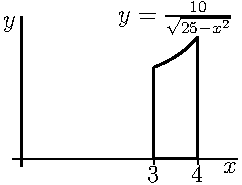
\includegraphics{graphE97D_3}
\end{center}


\noindent(b)
$\displaystyle10\pi\log\frac{9}{4}=20\pi\log\frac{3}{2}$
\qquad (c)
 $20\pi$
\end{answer}

\begin{solution} (a)
Let's graph $y=\dfrac{10}{\sqrt{25-x^2}}$.
We start with the endpoints: $(3,\frac{5}{2})$ and $(4,\frac{10}{3})$. Then we consider the first derivative:
\[\diff{}{x}\left\{\frac{10}{\sqrt{25-x^2}}\right\} = \frac{10x}{\sqrt{25-x^2}^3}\]

Over the interval $[3,4]$, this is always positive, so our function is increasing over the entire interval. The second derivative,

\[\ddiff{2}{}{x}\left\{\frac{10}{\sqrt{25-x^2}}\right\}=\diff{}{x}\left\{\frac{10x}{\sqrt{25-x^2}^3}\right\} = \frac{10(2x^2+25)}{\sqrt{25-x^2}^5},\]

is always positive, so our function is concave up over the entire interval. So,
the region $R$ is:

\begin{center}
       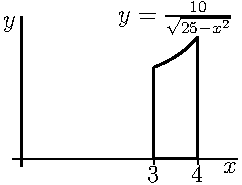
\includegraphics{graphE97D_3}
\end{center}




\noindent (b)
Let $\cV_1$ be the solid obtained by revolving
$R$ about the $x$--axis. The portion of $\cV_1$ with $x$--coordinate
between $x$ and $x+\dee{x}$ is obtained by rotating the red vertical strip in
the figure on the left below about the $x$--axis.
That portion is a disk of radius $\frac{10}{\sqrt{25-x^2}}$ and thickness
$\dee{x}$. The volume of this disk is $\pi\big(\frac{10}{\sqrt{25-x^2}}\big)^2\,\dee{x}$.
So the total volume of $\cV_1$ is
\begin{align*}
\int_3^4\pi{\Big(\frac{10}{\sqrt{25-x^2}}\Big)}^2\ \dee{x}
&=100\pi\int_3^4\frac{1}{25-x^2}\ \dee{x}
=100\pi\int_3^4\frac{1}{(5-x)(5+x)}\ \dee{x} \\
&=10\pi\int_3^4\Big(\frac{1}{5-x}+\frac{1}{5+x}\Big)\ \dee{x}
=10\pi\Big[-\log(5-x)+\log(5+x)\Big]_3^4 \\
&=10\pi\Big[-\log1+\log9+\log2-\log8\Big]
=10\pi\log\frac{9}{4}=20\pi\log\frac{3}{2}
\end{align*}

\begin{center}
       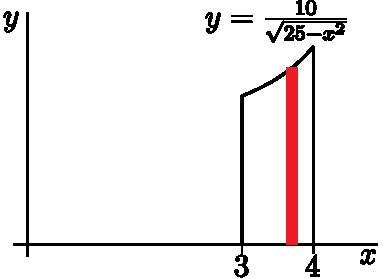
\includegraphics{graphE97D_3l}\qquad\qquad
       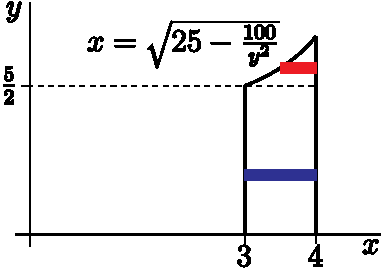
\includegraphics{graphE97D_3r}
\end{center}



\noindent (c)
We'll use horizontal washers as in Example  \eref{CLP101}{eg rot yaxis}
of the %\href{http://www.math.ubc.ca/%7Efeldman/m101/clp/clp_notes_101.pdf}{CLP-2 text}.
CLP-2 text.
 \begin{itemize}
\item We cut $\cR$ into thin horizontal  strips of width $\dee{y}$ as in
the figure on the right above.

\item When we rotate $\cR$ about the $y$--axis, each strip sweeps out a thin washer
\begin{itemize}
\item
whose outer radius is $r_{out}=4$, and
\item
whose inner radius is $r_{in}= \sqrt{25-\frac{100}{y^2}}$ when
$y\ge \frac{10}{\sqrt{25-3^2}} = \frac{10}{4}
=\frac{5}{2}$ (see the red strip in the figure on the right above),  and
whose inner radius is $r_{in}= 3$ when $y\le \frac{5}{2}$
(see the blue strip in the figure on the right above) and
\item
whose thickness is $\dee{y}$ and hence
\item
whose volume is
$\pi(r_{out}^2 - r_{in}^2)\dee{y} = \pi\big(\frac{100}{y^2}-9\big)\dee{y}$
when $y\ge \frac{5}{2}$ and  whose volume is
$\pi(r_{out}^2 - r_{in}^2)\dee{y} = 7 \pi\,\dee{y}$
when $y\le \frac{5}{2}$ and

\end{itemize}
\item As our bottommost strip is at $y=0$ and our topmost
strip is at $y=\frac{10}{3}$ (since at the top $x=4$ and $y=  \frac{10}{\sqrt{25-x^2}}
=\frac{10}{\sqrt{25-4^2}} =\frac{10}{3}$), the volume is
\begin{align*}
&\int _{5/2}^{10/3}  \pi\Big(\frac{100}{y^2}-9\Big)\dee{y}
                                                         +\int _ 0^{5/2}7 \pi\,\dee{y} \\
&=\pi{\Big[-\frac{100}{y}-9y\Big]}_{5/2}^{10/3} +\frac{35}{2}\pi\\
&=\pi \Big[-30+40-30+\frac{45}{2}\Big] +\frac{35}{2}\pi\\
&=20\pi
\end{align*}
\end{itemize}

\end{solution}
%%%%%%%%%%%%%%%%%%%



\begin{question}
Find the area of the finite region bounded by the curves $y=\dfrac{4}{3+x^2}$, $y=\dfrac{2}{x(x+1)}$, $x=\dfrac14$, and $x=3$.
\end{question}
\begin{hint}
You'll need to use two regions, because the curves cross.
\end{hint}
\begin{answer}
$\displaystyle2\log\frac53+\frac{4}{\sqrt3}\arctan\frac{1}{4\sqrt3}$
\end{answer}
\begin{solution}
In order to find the area between the curves, we need to know which one is on top, and which on the bottom. Let's start by finding where they meet.
\begin{align*}
\dfrac{4}{3+x^2}&=\frac{2}{x(x+1)}\\
2x^2+2x&=3+x^2\\
x^2+2x-3&=0\\
(x-1)(x+3)&=0
\end{align*}
In the interval $[\frac14,3]$, the curves only meet at $x=1$. So, to find which is on top and on bottom in the intervals $[\frac14,1)$ and $(1,3]$, it suffices to check some point in each interval.
\begin{center}
\begin{tabular}{|c||c|c||c|}
\hline
$x$ & $\frac{4}{3+x^2}$ & $\frac{2}{x(x+1)}$& Top:\\
\hline
$1/2$ &$16/13$ &$8/3$ &$\frac{2}{x(x+1)}$\\
\hline
$2$ &$4/7$ & $1/3$& $\frac{4}{3+x^2}$\\
\hline
\end{tabular}
\end{center}
So, $\frac{2}{x(x+1)}$ is the top function when $\frac{1}{4}\leq x < 1$, and
$\frac{4}{3+x^2}$ is the top function when $1<x \leq 3$. Then the area we want to find is:
\[\mbox{Area}=\int_{\frac14}^1 \left( \frac{2}{x(x+1)} - \frac{4}{3+x^2}\right)~\dee{x}+
\int_{1}^3 \left( \frac{4}{3+x^2} -\frac{2}{x(x+1)}  \right)~\dee{x} \]

We'll need to antidifferentiate both these functions. We can antidifferentiate $\dfrac{2}{x(x+1)}$ using partial fraction decomposition.

\begin{align*}
\frac{2}{x(x+1)}&=\frac{A}{x}+\frac{B}{x+1} = \frac{(A+B)x+A}{x(x+1)}\\
\color{red}A&\color{red}=2,\quad B=-2\\
\int\frac{2}{x(x+1)}~\dee{x}&=\int\left(\frac{2}{x}-\frac{2}{x+1}\right)~\dee{x}=2\log|x|-2\log|x+1|+C\\
&=2\log\left| \frac{x}{x+1}\right|+C
\end{align*}

We can antidifferentiate $\dfrac{4}{3+x^2}$ using the substitution $u=\frac{x}{\sqrt3}$, $\dee{u}=\frac{1}{\sqrt3}~\dee{x}$.
\begin{align*}
\int\frac{4}{3+x^2}~\dee{x}&=
\int\frac{4}{3\left(1+\left(\frac{x}{\sqrt3}\right)^2\right)}~\dee{x}=
\int\frac{4\sqrt3}{3\left(1+u^2\right)}~\dee{u}\\
&=\frac{4}{\sqrt3}\arctan u +C=\frac{4}{\sqrt3}\arctan \left(\frac{x}{\sqrt3}\right) +C
\end{align*}

Now, we can find our area.
\begin{align*}
\mbox{Area}&=\int_{\frac14}^1 \left( \frac{2}{x(x+1)} - \frac{4}{3+x^2}\right)~\dee{x}+
\int_{1}^3 \left( \frac{4}{3+x^2} -\frac{2}{x(x+1)}  \right)~\dee{x}\\
&=\left[2\log\left|\frac{x}{x+1}\right| - \frac{4}{\sqrt3}\arctan\left(\frac{x}{\sqrt3}\right)\right] _{1/4}^1+
\left[ \frac{4}{\sqrt3}\arctan\left(\frac{x}{\sqrt3}\right)-2\log\left|\frac{x}{x+1}\right|\right]_1^3\\
&=\left(2\log\frac{1}{2}- \frac{4}{\sqrt3}\cdot\frac{\pi}{6} - 2\log\frac{1}{5}+\frac{4}{\sqrt3}\arctan\frac{1}{4\sqrt3}\right)+\\
&\hphantom{=} \left(\frac{4}{\sqrt3}\cdot\frac{\pi}{3} - 2\log\frac34 - \frac{4}{\sqrt3}\cdot \frac{\pi}{6}+2\log\frac{1}{2}\right)\\
&=2\log\frac53+\frac{4}{\sqrt3}\arctan\frac{1}{4\sqrt3}
\end{align*}
\end{solution}
%%%%%%%%%%%%%%%%%%%


\begin{Mquestion} Let $F(x) = \displaystyle\int_1^x \frac{1}{t^2-9} \dee{t}$.
\begin{enumerate}[(a)]
\item
Give a formula for $F(x)$ that does not involve an integral.
\item Find $F'(x)$.
\end{enumerate}
\end{Mquestion}
\begin{hint}
For (b), use the Fundamental Theorem of Calculus Part 1.
\end{hint}
\begin{answer}
(a) $\displaystyle\frac{1}{6}\left(\log\left| 2\cdot\frac{x-3}{x+3} \right|\right)$
\qquad
(b) $F'(x) = \frac{1}{x^2-9}$
\end{answer}
\begin{solution}
(a) To antidifferentiate $\dfrac{1}{t^2-9}$, we use a partial fraction decomposition.
\begin{align*}
\frac{1}{t^2-9}&=\frac{1}{(t-3)(t+3)} = \frac{A}{t-3}+\frac{B}{t+3}=\frac{(A+B)t+3(A-B)}{(t-3)(t+3)}\\
A+B&=0,\quad A-B = \frac{1}{3}\\
\color{red}A&\color{red}=\frac{1}{6},\quad B = -\frac{1}{6}\\
F(x)&=\int_1^x\frac{1}{t^2-9}~\dee{x} =
\int_1^x \left(\frac{1/6}{t-3}-\frac{1/6}{t+3}\right)~\dee{x}\\
&=\left[\frac{1}{6}\log|t-3| - \frac{1}{6}\log|t+3|\right]_1^x\\
&=\left(\frac{1}{6}\log|x-3| - \frac{1}{6}\log|x+3|
-\frac{1}{6}\log2 +\frac{1}{6}\log4\right)\\
&=\frac{1}{6}\left(\log\left| 2\cdot\frac{x-3}{x+3} \right|\right)
\end{align*}

(b) Rather than differentiate our answer from (a), we use the Fundamental Theorem of Calculus Part 1 to conclude \[F'(x) = \diff{}{x}\left\{ \displaystyle\int_1^x \frac{1}{t^2-9} \dee{t}\right\} = \frac{1}{x^2-9}\]
\end{solution}


%%%%%%%%%%%%%%%%%%%


%%%%%%%%%%%%%%%%%%%
